\DocumentMetadata{
  pdfversion=2.0,
  lang=es-MX,
  pdfstandard=ua-2
}

\documentclass{sener2025}

\addbibresource{referencias.bib}

% --- Metadatos PDF/UA (Accesibilidad Universal) ---
\hypersetup{
  pdftitle={Documento DEMO — Plantilla SENER LaTeX},
  pdfauthor={Equipo de Planeación (demo)},
  pdfsubject={Ejemplos de secciones, etiquetas y bloques (para pruebas del generador)},
  pdfkeywords={demo; plantilla; secciones; etiquetas; tablas; figuras},
  pdfcreationdate={D:20251216175902},
  pdfversion={1}
}

% --- Metadatos del Documento ---
\title{Documento DEMO — Plantilla SENER LaTeX}
\subtitle{Ejemplos de secciones, etiquetas y bloques (para pruebas del generador)}
\author{Equipo de Planeación (demo)}
\date{14 de diciembre de 2025}
\institucion{Secretaría de Energía (SENER)}
\unidad{Unidad de Planeación y Transición Energética}
\setDocumentoCorto{DEMO\_SENER\_SASSO}
\palabrasclave{demo; plantilla; secciones; etiquetas; tablas; figuras}
\version{1}

\begin{document}

\portadafondo[img/portada.png]

\tableofcontents
\newpage

\listafiguras
\newpage

\listatablas
\newpage

\clearpage
\begin{center}
{\Large\patriafont\bfseries\color{gobmxGuinda}Agradecimientos}\\[1cm]
\end{center}

Agaredecemos a:
1.-JAvi
2.-Diego
3.-Rodrigo

\clearpage
\begin{center}
{\Large\patriafont\bfseries\color{gobmxGuinda}Presentación}\\[1cm]
\end{center}

ESto es un texot de presemntacion ..... bka....bla...blan

\clearpage
\begin{center}
{\Large\patriafont\bfseries\color{gobmxGuinda}Resumen Ejecutivo}\\[1cm]
\end{center}

Este documento es un banco de pruebas. Incluye ejemplos de:
• Listas
• Etiquetas inline (nota, cita, math)
• Bloques (recuadro, ejemplo, info, alerta)
• Anexos
• Tablas y figuras

Objetivo: detectar errores de escape y de parsing antes de publicar.

\clearpage
\begin{center}
{\Large\patriafont\bfseries\color{gobmxGuinda}Datos Clave}\\[1cm]
\end{center}

\begin{itemize}
  \item Dato 1
  \item Dato 2
  \item Dato 3
  \item Dato 4
\end{itemize}

\portadaseccion{1}{Capítulo 1}{Guía rápida (etiquetas + bloques)}

\section{Guía rápida de sintaxis}

Este párrafo muestra texto normal con acentos (México, energía, transición).
También prueba caracteres especiales que deben escaparse: 100\% , \$1,234 , \& , \_ , \# , \{ \} .

Ejemplo de nota al pie: La demanda eléctrica crece de forma sostenida\footnote{Nota al pie desde Sheets/Excel. Soporta texto largo y símbolos como \% y \&.}.
Ejemplo de cita bibliográfica: ver \cite{demo_sener2025} y \cite{cenace2023_flex}.

Inline math: El coeficiente de potencia es $C_p$ y la eficiencia $\eta = \frac{P_{out}}{P_{in}}$.
Display equation (sin escapar comandos dentro):
\begin{equation}
\eta = \frac{P_{out}}{P_{in}}
\end{equation}

Lista simple (una línea = un item):
\begin{itemize}
  \item Primer punto con \textbf{\textcolor{gobmxDorado}{énfasis dorado}}
  \item Segundo punto con \textbf{\textcolor{gobmxGuinda}{énfasis guinda}}
  \item Tercer punto con referencia a tabla/figura (opcional)
\end{itemize}
Aquí va una Figura:
% Referencia a figura: FIG-1-1

Prueba de saltos como texto literal: escribe

 en una celda y asegúrate que el pipeline lo convierta en salto real (esto es un test).

\cite{bne2024_generacion}

Tabla test:
% Referencia a tabla: TBL-1-1
\begin{tabladoradoCorto}
  \caption{Javi tablas}
  \label{tab:TBL-1-1}
  \begin{tabular}{H{3cm}G{2cm}}
    \toprule
    \rowcolor{gobmxDorado} \encabezadodorado{\textbf{Concepto}} & \encabezadodorado{Encabezado} \\
    \midrule
    \textbf{Javi} & Prueba \\
    \bottomrule
  \end{tabular}
\end{tabladoradoCorto}

\begin{figure}[H]
  {\centering
  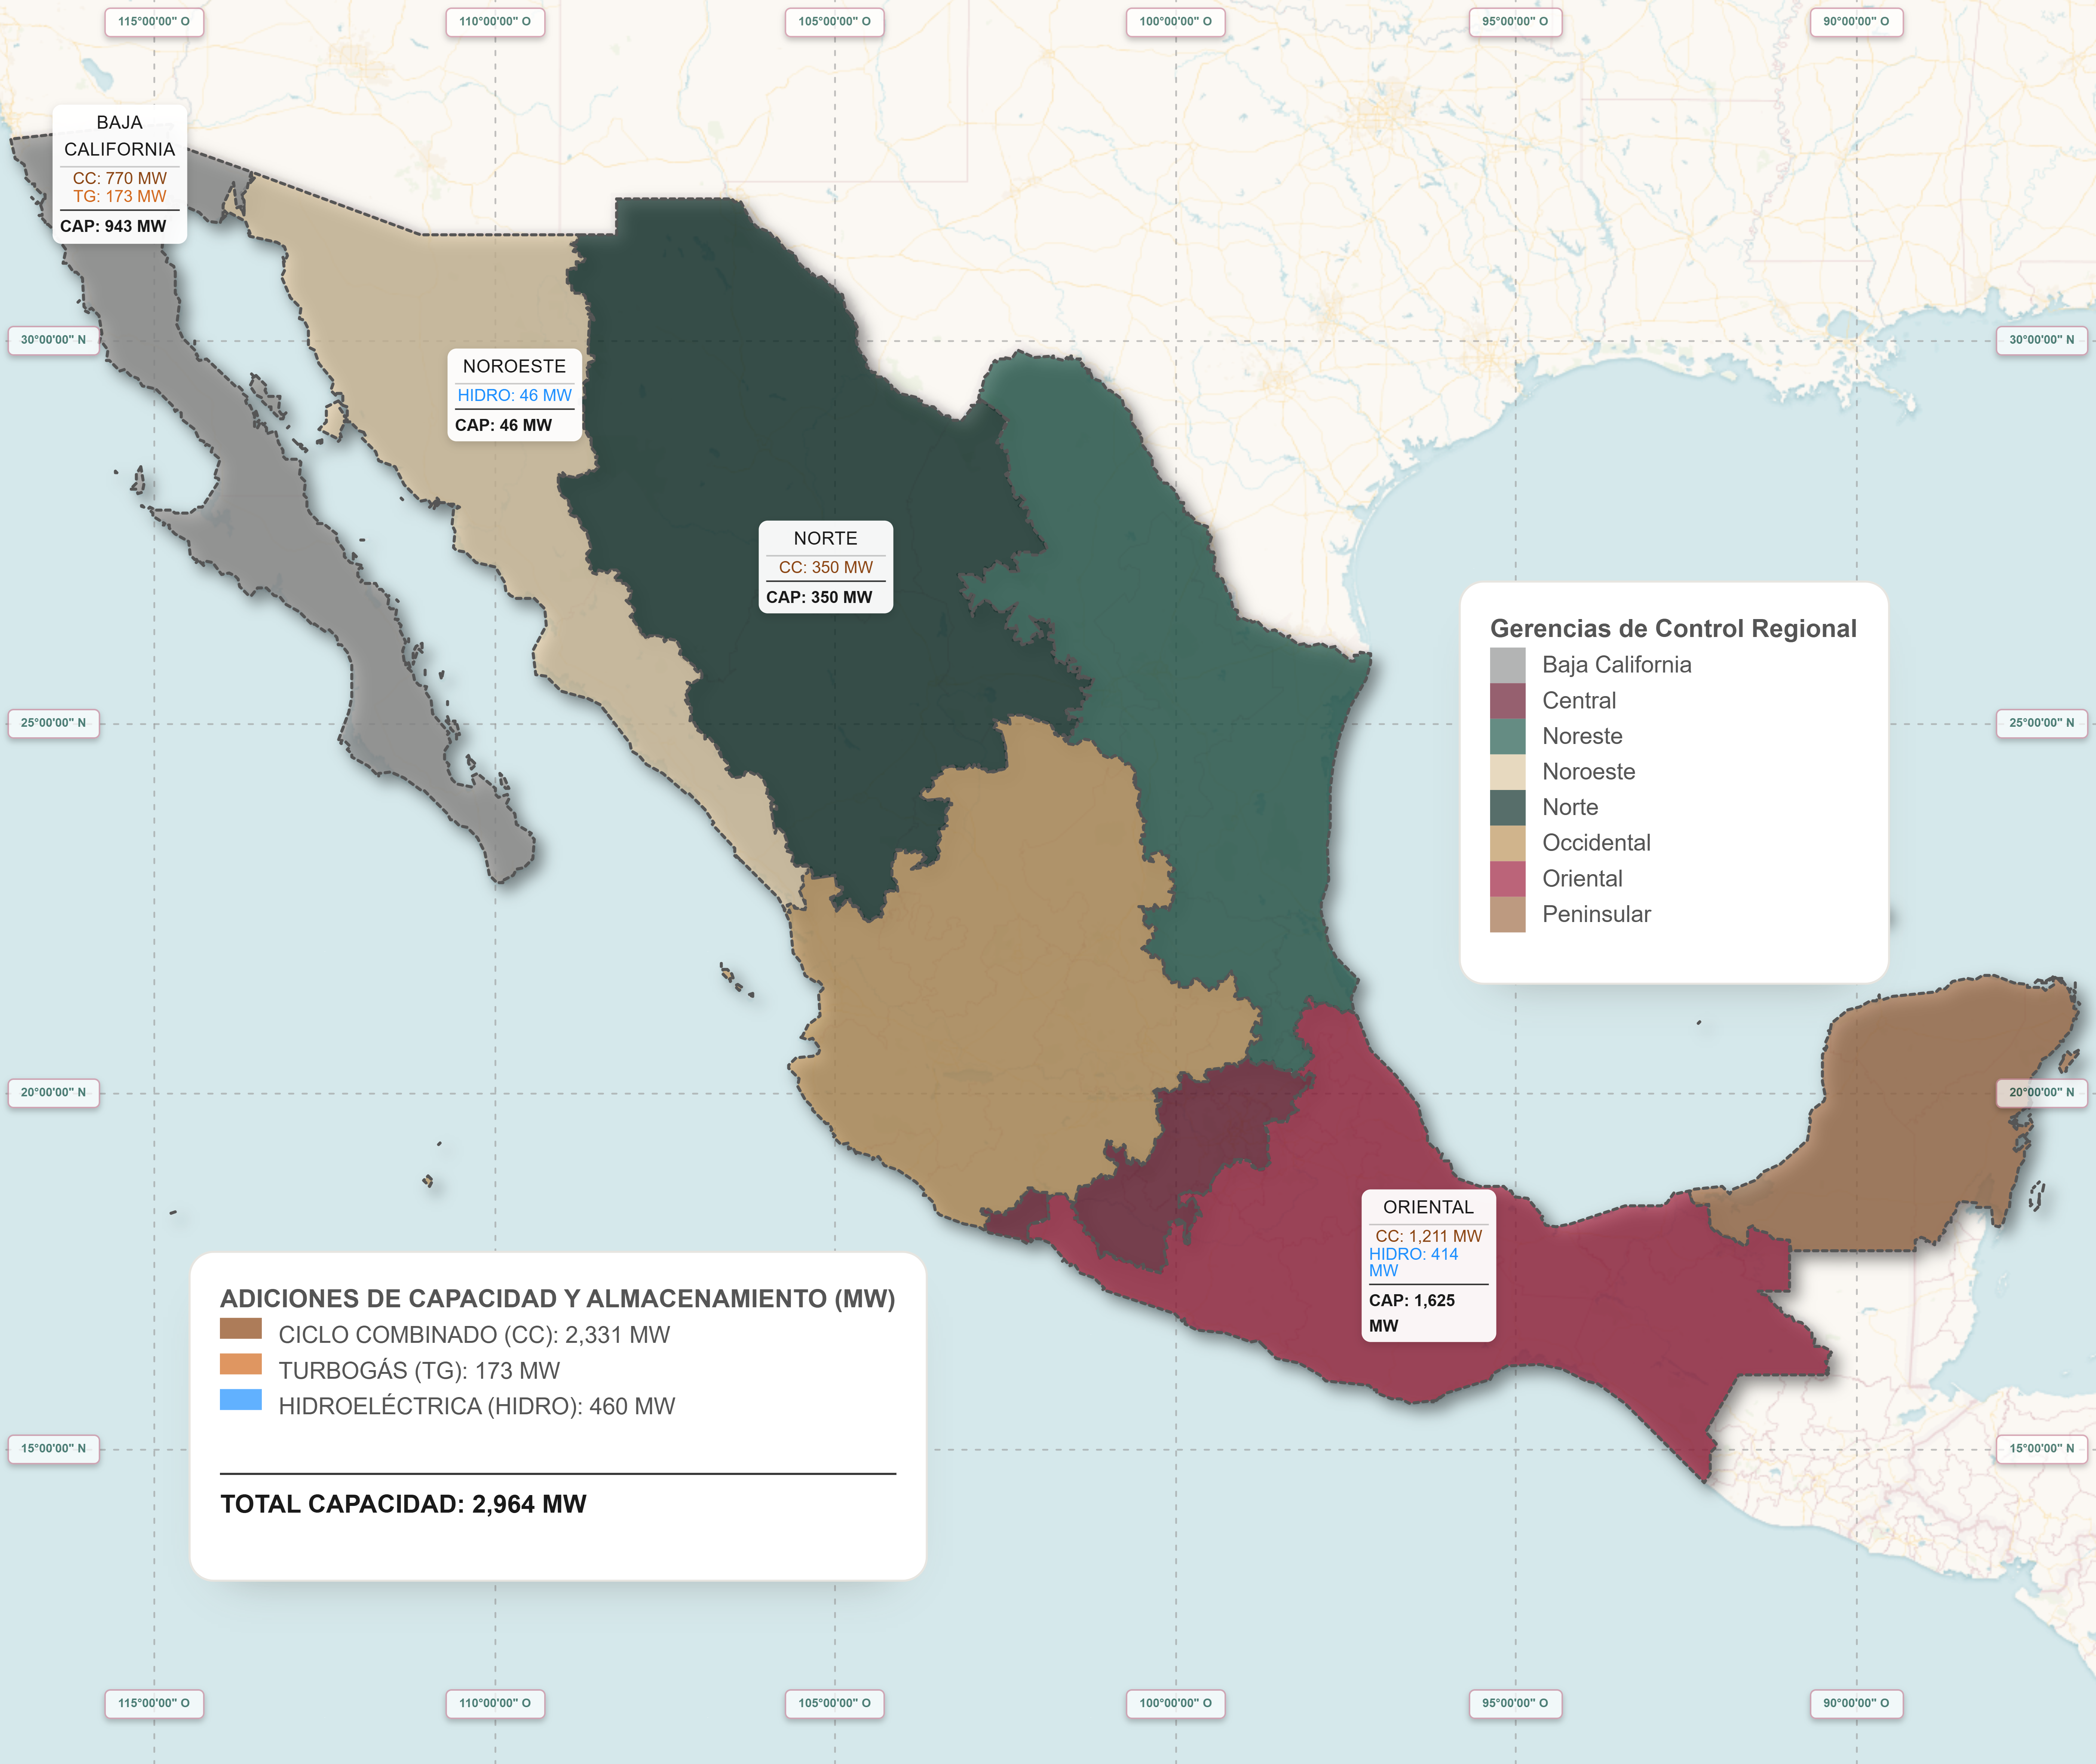
\includegraphics[width=0.8\textwidth]{img/graficos/figura_4_3.png}
  \par}
  \raggedright
\end{figure}



\subsection{Etiquetas inline (dentro de un párrafo)}

Puedes mezclar etiquetas dentro de texto:
\begin{itemize}
  \item \textbf{\textcolor{gobmxDorado}{Texto dorado}} y \textbf{\textcolor{gobmxGuinda}{Texto guinda}}
  \item Nota al pie: \footnote{Una nota corta.}
  \item Citas: \cite{demo_sener2025}
  \item Math inline: $E = mc^2$
\end{itemize}
Recomendación: usa estas etiquetas inline SOLO para fragmentos cortos. Para cajas completas usa bloques.


\subsection{Bloques (cajas) usando líneas separadas}

Los bloques deben ir en líneas separadas, así:

\begin{recuadro}[title={Nota metodológica}]
Este recuadro acepta varias líneas.
También acepta listas:
\begin{itemize}
  \item Item A
  \item Item B con \textbf{\textcolor{gobmxDorado}{resaltado}}
\end{itemize}
\end{recuadro}

\begin{ejemplo}[title={Ejemplo de cálculo}]
Si P es potencia y V voltaje, entonces:
\begin{equation}
P = V\cdot I
\end{equation}

\end{ejemplo}

\begin{calloutTip}
Tip: usa $\Delta$ para deltas y $\%$ no es necesario (el generador debe escapar \% en texto normal).

\end{calloutTip}

\begin{calloutWarning}
Advertencia: si escribes comandos LaTeX crudos (\textbackslash\{\}begin, \textbackslash\{\}textbf, etc.) el generador los escapará a menos que tengas una etiqueta especial para 'raw'.

\end{calloutWarning}


\section{Tablas y figuras (inserción automática)}

Esta sección está pensada para probar que el generador inserta automáticamente:
\begin{itemize}
  \item 1 figura asociada con SeccionOrden=2.0 (ver hoja 'Figuras').
  \item 2 tablas asociadas con SeccionOrden=2.0 (ver hoja 'Tablas' y rangos en 'Datos Tablas').
\end{itemize}
Si quieres referenciar explícitamente en texto, puedes poner comentarios:


\section{Prueba de párrafos y saltos de línea}

Este es el párrafo 1.

Este es el párrafo 2 (separado por una línea en blanco).

Ahora una lista:
\begin{itemize}
  \item Línea 1
  \item Línea 2
\end{itemize}
Fin.


\paragraph{Mini encabezado dentro de sección}

c


\anexos

\section{Ejemplo de anexo}

El primer nivel que contenga 'anexo' debe activar \textbackslash\{\}anexos (numeración alfabética).

\begin{recuadro}[title={Anexo — notas}]
Contenido dentro de anexo.

\end{recuadro}


\subsection{Detalle adicional}

Subanexo (mapea a \textbackslash\{\}subsection en modo anexos).


\section*{Glosario}
\phantomsection
\addcontentsline{toc}{section}{Glosario}

\entradaGlosario{Eficiencia energética}{Relación entre la energía útil obtenida y la energía consumida para lograr un servicio.}
\entradaGlosario{Energías renovables variables}{Tecnologías cuya generación depende del recurso (viento, solar) y fluctúa en el tiempo.}
\entradaGlosario{Flexibilidad del sistema}{Capacidad del sistema eléctrico para responder a variaciones de oferta/demanda, especialmente con renovables variables.}

\printbibliography

\section*{Siglas y Acrónimos}
\phantomsection
\addcontentsline{toc}{section}{Siglas y Acrónimos}

\entradaSigla{CENACE}{Centro Nacional de Control de Energía}
\entradaSigla{CRE}{Comisión Reguladora de Energía}
\entradaSigla{SENER}{Secretaría de Energía}

\paginacreditos{
\begin{center}
{\patriafont\fontsize{12}{14}\selectfont\color{gobmxGuinda} Nombre Apellido Apellido}\\
{\patriafont\fontsize{9}{11}\selectfont Cargo o puesto}\\[0.5cm]
{\patriafont\fontsize{12}{14}\selectfont\color{gobmxGuinda} Nombre 2 Apellido 2}\\
{\patriafont\fontsize{9}{11}\selectfont Cargo 2}\\[0.5cm]
\end{center}
}
\contraportada[img/contraportada.png]{
\textbf{\textcolor{gobmxDorado}{ Elaboración:}}\\
Dirección General (demo)\\[0.5cm]
\textbf{\textcolor{gobmxDorado}{ Contacto:}}\\
correo@ejemplo.gob.mx\\[0.5cm]
\textbf{\textcolor{gobmxGuinda}{ www.gob.mx/sener}}
}

\end{document}
